%% 
%% Copyright 2007-2019 Elsevier Ltd
%% 
%% This file is part of the 'Elsarticle Bundle'.
%% ---------------------------------------------
%% 
%% It may be distributed under the conditions of the LaTeX Project Public
%% License, either version 1.2 of this license or (at your option) any
%% later version.  The latest version of this license is in
%%    http://www.latex-project.org/lppl.txt
%% and version 1.2 or later is part of all distributions of LaTeX
%% version 1999/12/01 or later.
%% 
%% The list of all files belonging to the 'Elsarticle Bundle' is
%% given in the file `manifest.txt'.
%% 

%% Template article for Elsevier's document class `elsarticle'
%% with numbered style bibliographic references
%% SP 2008/03/01
%%
%% 
%%
%% $Id: elsarticle-template-num.tex 168 2019-02-25 07:15:41Z apu.v $
%%
%%
\documentclass[preprint,12pt]{elsarticle}

%% Use the option review to obtain double line spacing
%% \documentclass[authoryear,preprint,review,12pt]{elsarticle}

%% Use the options 1p,twocolumn; 3p; 3p,twocolumn; 5p; or 5p,twocolumn
%% for a journal layout:
%% \documentclass[final,1p,times]{elsarticle}
%% \documentclass[final,1p,times,twocolumn]{elsarticle}
%% \documentclass[final,3p,times]{elsarticle}
%% \documentclass[final,3p,times,twocolumn]{elsarticle}
%% \documentclass[final,5p,times]{elsarticle}
%% \documentclass[final,5p,times,twocolumn]{elsarticle}

%% For including figures, graphicx.sty has been loaded in
%% elsarticle.cls. If you prefer to use the old commands
%% please give \usepackage{epsfig}

%% The amssymb package provides various useful mathematical symbols
\usepackage{amssymb}
%% The amsthm package provides extended theorem environments
%% \usepackage{amsthm}

%% The lineno packages adds line numbers. Start line numbering with
%% \begin{linenumbers}, end it with \end{linenumbers}. Or switch it on
%% for the whole article with \linenumbers.
%% \usepackage{lineno}

\journal{journal X}

\begin{document}

\begin{frontmatter}

%% Title, authors and addresses

%% use the tnoteref command within \title for footnotes;
%% use the tnotetext command for theassociated footnote;
%% use the fnref command within \author or \address for footnotes;
%% use the fntext command for theassociated footnote;
%% use the corref command within \author for corresponding author footnotes;
%% use the cortext command for theassociated footnote;
%% use the ead command for the email address,
%% and the form \ead[url] for the home page:
%% \title{Title\tnoteref{label1}}
%% \tnotetext[label1]{}
%% \author{Name\corref{cor1}\fnref{label2}}
%% \ead{email address}
%% \ead[url]{home page}
%% \fntext[label2]{}
%% \cortext[cor1]{}
%% \address{Address\fnref{label3}}
%% \fntext[label3]{}

\title{CV for anomaly detection in industrial applications}

%% use optional labels to link authors explicitly to addresses:
%% \author[label1,label2]{}
%% \address[label1]{}
%% \address[label2]{}

\author{Viacheslav Kozitsin, Iurii Katser, Arman Alahyari, Anton Hinneck, Rahim Tariverdi}

\address{Skolkovo Institute of Science and Technology}

\begin{abstract}
%% Text of abstract

\end{abstract}

%%Graphical abstract
%\begin{graphicalabstract}
%%\includegraphics{grabs}
%\end{graphicalabstract}

%%Research highlights
%\begin{highlights}
%	\item Research highlight 1
%	\item Research highlight 2
%\end{highlights}

\begin{keyword}
%% keywords here, in the form: keyword \sep keyword
deep learning \sep computer vision \sep anomaly detection \sep fault detection \sep technical systems
%% PACS codes here, in the form: \PACS code \sep code

%% MSC codes here, in the form: \MSC code \sep code
%% or \MSC[2008] code \sep code (2000 is the default)

\end{keyword}

\end{frontmatter}

%% \linenumbers

%% main text
\section{INTRODUCTION}
\label{INTRODUCTION}

Anomaly detection problems have a great importance in industrial applications, because anomalies usually represent faults, failures or the emergence of such. To detect these automatically, we propose deep learning algorithms for anomaly / fault detection and their classification. We develop an algorithm achieving Segmentation Defects classification Its performance will be examined on two different problems: anomaly detection in oil pipelines and fault detection on transmission system components. Both these systems can span over thousands of kilometers, which makes manual inspection very costly. How such computer vision techniques can be applied on an industrial scale is discussed in the following.

Transmission infrastructure, on the other hand, physically connects power sources and consumers extending over thousands of kilometers. Many different components exist, which is why maintaining power grids is a serious cost factor for transmission system operators (TSOs). Automated fault detection could potentially help to decrease costs. To use an automated visual system however, specific infrastructure first needs to be identified and segmented, to then perform any type of fault detection. Therefore, the proposed deep learning-based approach, to segment and identify faulty components (i.e. insulators) in handheld footage, will be tested regarding its viability. If a deep-learning based approach would prove reliable, drones could monitor equipment automatically.

The damage of pipelines that transport petroleum and gas products lead to severe environmental problems. Eliminating breakthroughs and their consequences is expensive. To avoid accidents, it is recommended to improve diagnostics quality and to increase the frequency of in-line-inspection (ILI) tools deployment. ILI tools, also referred to as pipeline inspection gauges (Fig.~\ref{ris:ili}), use Hall effect for measuring localized magnetic flux leakage intensity along the pipe wall. While moving along the pipe gauge inspects the wall and detects the magnetic field leaks.
\begin{figure}[ht]
	\center{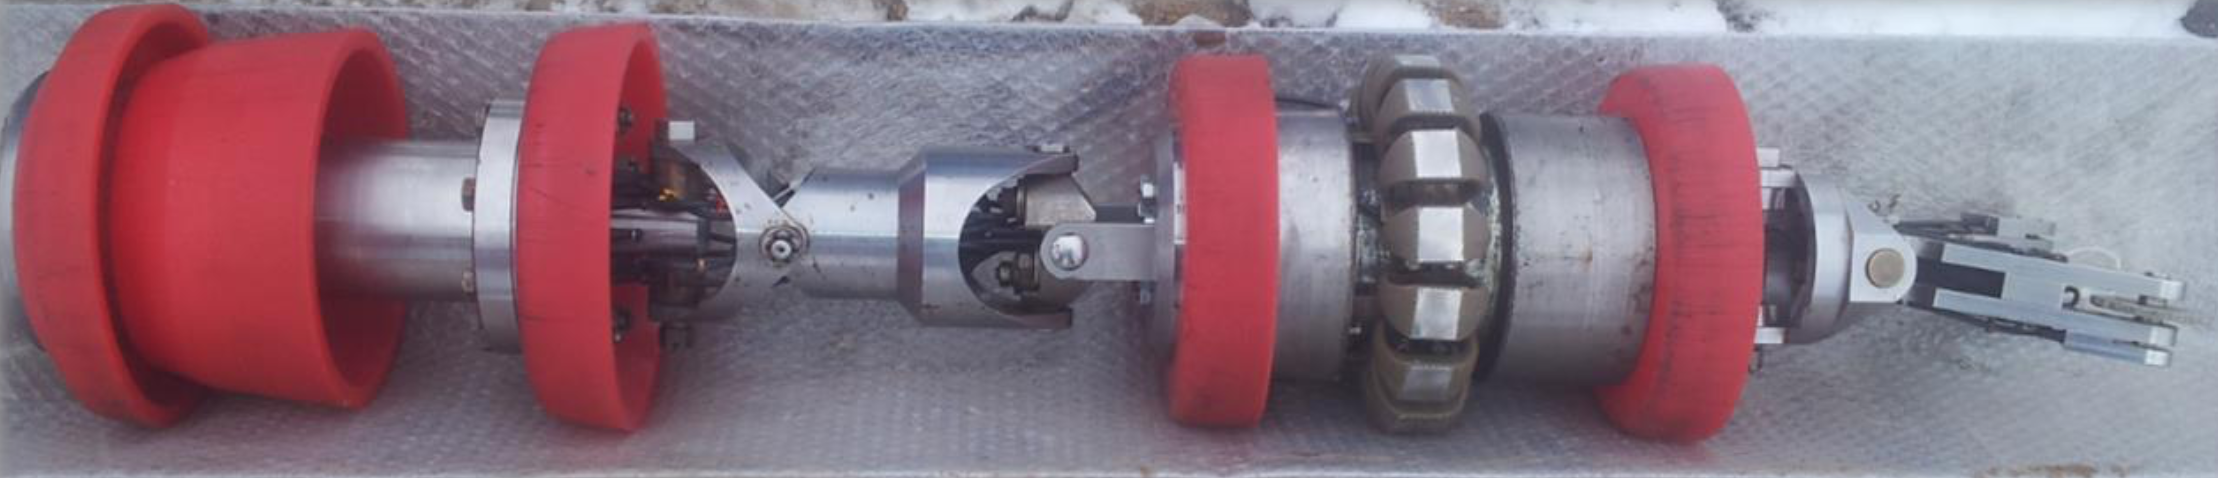
\includegraphics[scale=0.35]{pictures/ili.png}}
	\caption{In-line-inspection tool}
	\label{ris:ili}
\end{figure}
The data collected during the inspection can be further analyzed for main diagnostics problems solving: damage and defects detection, their localization, diagnosis or defects classification.
Analysis results are usefull for assets managing and repair priorities determination.

\section{LITERATURE REVIEW}
\label{LITERATURE REVIEW}

\subsection{Pipelines defects diagnostics}

Magnetic Flux Leakage (MFL) technique is the most common approach for oil and gas pipelines nondestructive testing.
The data obtained during the pipeline inspection process is primarily analyzed by traditional machine learning (ML) methods.
A comparison of performance among different ML methods for defects identification problem is presented in \cite{Khodayari-Rostamabad2009}.
The main challenge for this approach is creating informative and important features that will be used as an input for ML methods.
Usually, these diagnostics features are generated using expert knowledge and manually-created heuristics.
It imposes the limitation on defects detection problem solving quality.
A variety of most successful features is presented and analyzed in details in \cite{Slesarev2017}.

Deep Learning showed significant progress and achieved incredible results in numerous applications, just in the past few years.
The image classification problem is one of the most successful applications of DL and Convolutional Neural Networks (CNNs) in particular.
To automate the process of feature generation in MFL data analysis, CNNs can be used either.
As an advantage, they can solve the defects detection and segmentation tasks at the same time.
In literature there are examples of applying CNNs for defects detection \cite{Feng2017}, welds defect detection \cite{2020a}, welds and defects classification \cite{Yang2020}, defect size estimation \cite{Lu2019}.
For all mentioned applications, CNNs outperformed existing traditional approaches.
Nevertheless, still, there are just a few works dedicated to MFL data analysis using DL.
A number of particular problems that can be solved using a novel approach are not covered yet.
For instance, we could not find any works on applying CNNs to defects segmentation task, despite the importance of this problem solving according to \cite{Feng2017}.

In this work, we want to research two different problems:
\begin{enumerate}
	\item Defects detection (Picture classification task).
	\item Defects segmentation (Semantic segmentation task).
\end{enumerate}

For their solving, we propose CNNs of different architectures and compare their results with existing state-of-the-art approaches.
Moreover, we research different preprocessing techniques for dealing with typical issues in the MFL data.
\subsection{Unet}
\section{CONTRIBUTION}
\label{CONTRIBUTION}

\paragraph{Viacheslav Kozitsin}
The main task was to solve problem of semantic segmentation of defects in pipes.  Outcomes: A baseline was chosen as a stripped-down version of UNet (Figure \ref{ris:UNet}). The specifics of applying UNet under conditions of small sizes of the original image (64x64) were investigated. As a result, the problem was solved with IoU=0.2 and good visual results (Figure\ref{ris:mainresult}). Concomitant successes: annotated the data for the defect segmentation of pipe (Table \ref{tab:alg1}); proposed own approach to the preprocessing of raw data from sensors based on expert knowledge (Figure \ref{ris:preproc_fun}); solved the problem of displaced origins between data and report files (Figure\ref{ris:prepr}). Active participation in the filling of the report and presentation. 

\paragraph{Iurii Katser}
The main task was to solve the defects detection problem for the oil pipeline dataset.
Exploratory Data Analysis (EDA) was provided.
EDA allowed us to define issues in data that impede CV problems solving without data preprocessing.
Data preprocessing tools were implemented (abnormal values filling, defects, and welds coordinates searching).
The influence of different preprocessing algorithms was analyzed and presented in the results section.
The CNN that overperformed the best existing network on the presented pipelines dataset was proposed.
Outcomes and future work were marked.
	
\paragraph{Arman Alahyari}
	
\paragraph{Anton Hinneck}
	
\paragraph{Rahim Tariverdi}
\section{METHODS PIPELINES}
\label{METHODS PIPELINES}

\section{RESULTS PIPELINES}
\label{RESULTS PIPELINES}

We present the results of comparison for different preprocessing techniques and different CNN architectures for binary classification (normal pipe wall or defect/weld) in Tab.~\ref{tab:comp1} and multiclass classification problem (normal pipe wall, defect or weld) in Tab.~\ref{tab:comp2}.

Batch size is equal to 64, so the input to the network has shape (64, 1, 64, 64).
For all experiments, we use Adam optimizer with initial learning rate 0.001 and learning rate scheduler with parameters: threshold = 0.0001, factor = 0.5, min lr = 0.0001, patience = 484.
Also, for all experiments, the number of epochs is equal to 12.
Dropout rate for all experiments is equal to 0.33.
All mentioned parameters were selected by using grid search procedure.

\begin{table}[!htb]
	\caption{\label{tab:comp1}Comparison of performance among different classification methods for binary classification problem}
	\begin{center}
		\small
		\begin{tabular}{| l | c | c | c |}
			\hline
			Method & $\hat{y}=y=0$ (normal) & $\hat{y}=y=1$ (defect/weld)  & Average \\
			\hline
			CNN-2 & 95.55 & 82.08 & 89.88 \\
			CNN-5 & 97.95 & \textbf{91.51} & \textbf{95.24} \\
			CNN-5+LRN & \textbf{98.29} & 89.86 & 94.74 \\
			\hline
			\multicolumn{4}{|c|}{Filling techniques comparison}  \\
			\hline
			CNN-5 (filling 1) & 97.95 & \textbf{91.51} & \textbf{95.24} \\
			CNN-5 (filling 2) & 97.95 & 84.20 & 92.16 \\
			CNN-5 (filling 3) & 97.26 & 83.02 & 91.27 \\
			CNN-5 (filling 4) & \textbf{98.63} & 81.13 & 91.27 \\
			CNN-5 (filling 5) & 98.12 & 81.84 & 91.27 \\
			\hline
			\multicolumn{4}{|c|}{Centering influence for the first filling method} \\
			\hline
			CNN-5 (centered) & 97.95 & \textbf{91.51} & 95.24 \\
			CNN-5 (not centered) & \textbf{98.46} & 91.27 & \textbf{95.44} \\
			CNN-2 (centered) & 95.55 & 82.08 & 89.88 \\
			CNN-2 (not centered) & 96.92 & 80.42 & 89.81 \\
			\hline
			\multicolumn{4}{|c|}{Image min-max normalization vs Whole dataset min-max normalization} \\
			\hline
			CNN-5 (centered) &  & &  \\
			CNN-5 (not centered) &   &  &  \\
			CNN-2 (centered) &  &  &  \\
			CNN-2 (not centered) &  &  &  \\
			\hline
		\end{tabular}
	\end{center}
\end{table}

Filling methods were researched for binary classification problem.
Centering means using peaks (extremums) searching procedure for welds or defects correct coordinates defining.
The centering procedure was research both for binary and multiclass classification problems.
Moreover, Min-Max normalization using either a single image or whole dataset was investigated.
Finally, CNN-2 and CNN-5 were compared for centered images with the first filling method using single image Min-Max normalization.

\begin{table}[!htb]
	\caption{\label{tab:comp2}Comparison of performance among different classification methods for multiclass classification problem}
	\begin{center}
		\small
		\begin{tabular}{| l | c | c | c | c |}
			\hline
			Method & $\hat{y}=y=0$ (normal) & $\hat{y}=y=1$ (defect) & $\hat{y}=y=2$ (weld) & Average \\
			\hline
			CNN-2 & 97.60 & 59.86 & 92.91 & 90.97 \\
			CNN-5 & \textbf{98.12} & \textbf{76.76} & \textbf{98.23} & \textbf{95.14} \\
			\hline
			\multicolumn{5}{|c|}{Centering influence for the first filling method}  \\
			\hline
			CNN-5 (centered) & \textbf{98.12} & \textbf{85.21} & 75.18 & 89.88 \\
			CNN-5 (not centered) &  \textbf{98.12} & 76.76 & \textbf{98.23} & \textbf{95.14} \\
			CNN-2 (centered) & 96.75 & 71.13 & 52.13 & 80.65 \\
			CNN-2 (not centered) & 97.60 & 59.86 & 92.91 & 90.97 \\
			\hline
			\multicolumn{5}{|c|}{Single image min-max normalization vs Whole dataset min-max normalization}  \\
			\hline
			CNN-5 (1) (whole) & 97.95 & 64.08 & \textbf{99.65} & 93.65 \\
			CNN-5 (1) (image) &  98.12 & \textbf{76.76} & 98.23 & \textbf{95.14} \\
			CNN-2 (1) (whole) & \textbf{99.32} & 13.38 & 96.45 & 86.41 \\
			CNN-2 (1) (image) & 97.60 & 59.86 & 92.91 & 90.97 \\
			CNN-5 (3) (whole) & 99.66 & 81.69 & 99.65 & 97.12 \\
%			CNN-5 (3) (image) &  98.12 & \textbf{76.76} & 98.23 & \textbf{95.14} \\
			CNN-2 (3) (whole) & 95.72 & 13.38 & 97.52 & 89.58 \\
%			CNN-2 (3) (image) & 97.60 & 59.86 & 92.91 & 90.97 \\
			\hline
		\end{tabular}
	\end{center}
\end{table}

\section{RESULTS PIPELINES}
\label{RESULTS PIPELINES}

\subsection
\section{CONCLUSION}
\label{CONCLUSION}
%TODO magnetographic image
Today, manual analysis of a magnetographic image is a bottleneck for the diagnosis of pipeline transport, since it costs a lot of money and is limited by human resources. This study allows us to hope that this process can be fully automated, which is likely to make the analysis more reliable, faster and cheaper.


%% The Appendices part is started with the command \appendix;
%% appendix sections are then done as normal sections
%% \appendix

%% \section{}
%% \label{}

%% If you have bibdatabase file and want bibtex to generate the
%% bibitems, please use
%%
\bibliographystyle{elsarticle-num} 
\bibliography{biblio}

%% else use the following coding to input the bibitems directly in the
%% TeX file.

%\begin{thebibliography}{00}
%
%%% \bibitem{label}
%%% Text of bibliographic item
%
%\bibitem{}
%
%\end{thebibliography}
\end{document}
\endinput
%%
%% End of file `elsarticle-template-num.tex'.
